\subsubsection{Surge tanks}

A surge tank is an open topped vessel, filled with fluid upto some predetermined height, as shown in figure \ref{fig:surge_tank_diagram}. By damping the pressure response and supplying/storing fluid a surge tank is often able to alleviate the ill effects of transient flows in a system {\color{red} Reference Chaudry p349-350}. Surge tanks are able to be modelled by modifying the consumption term in the continuity equation at a node thereby modifying the rate at which the nodal head changes with time. 

\begin{figure}
\centering
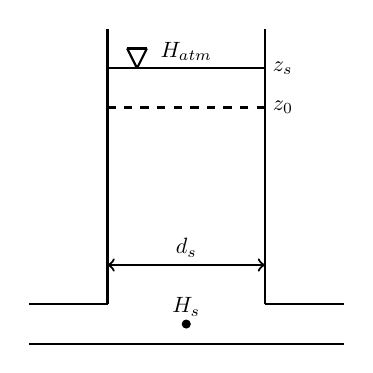
\begin{tikzpicture}[ scale=1, every node/.style={scale=0.8},] 
% Pipe
\draw[thick] (2,0) -- (-2,0);
\draw[thick] (1,0.5) -- (2,0.5);
\draw[thick] (-1,0.5) -- (-2,0.5);
% Sides
\draw[thick] (1,0.5) -- (1,4);
\draw[thick] (-1,0.5) -- (-1,4);
% Water levels
\draw[thick, dashed] (1,3) -- (-1,3);
\draw[thick] (1,3.5) -- (-1,3.5);


% Annotations
\node[anchor=west] at (1,3.5) {$z_s$};
\node[anchor=west] at (1,3) {$z_0$};
\node[anchor=south] at (0,1) {$d_s$};
\draw[thick, <->] (1,1) -- (-1,1);

% Node labels
\draw[fill=black] (0,0.25) circle (0.05cm);
\node[anchor=south] at (0,0.25) {$H_s$};
%\draw[fill=black] (0,3.5) circle (0.05cm);
\node[anchor=south] at (0,3.5) {$H_{\text{atm}}$};
% Free surface symbol
\draw[thick] (-0.5,3.75) -- (-0.75,3.75);
\draw[thick] (-0.5,3.75) -- (-0.625,3.5);
\draw[thick] (-0.75,3.75) -- (-0.625,3.5);
\end{tikzpicture} 
\caption{A surge tank boundary at node $s$ with an a fluid level $z_s$, an initial fluid level $z_0$ and tank diameter $d_s$.}
\label{fig:surge_tank_diagram}
\end{figure}

Suppose that a surge tank is placed in the network at node $s$, at this node we have the continuity equation
\begin{align}
\left( \mathbf{K}^T \right)_s \mathbf{Q} + D_{s,s} \pardiv{}{H_s}{t} = C_s,
\end{align}
where $\left( \mathbf{K}^T \right)_s$ indicates the $s$th row of the matrix $\mathbf{K}^T$ and $D_{s,s}$ indicates the element of the matrix $D$ at row $s$ and column $s$. The flow which leaves the node and fills the surge tank may be modelled by choosing an appropriate expression for the consumption term $C_s$. 

The nodal head $H_s$ is equal to the head due to atmospheric pressure plus the fluid column height i.e.
\begin{align}
H_s = H_{\text{atm}} + z_s.
\end{align} 
The rate at which fluid flows into the surge tank is
\begin{align*}
A_s \frac{d z_s}{d t},
\end{align*}
where $A_s = \pi d_s^2 / 4$ is the cross-sectional area of the tank. If we assume that the fluid in the tank moves as a slug then we may say that
 \begin{align*}
A_s \frac{d z_s}{d t} = A_s \pardiv{}{z_s}{t} = A_s \pardiv{}{H_s}{t}.
\end{align*}
Therefore, since flow into the tank is equal to flow out of the node $(C_s < 0)$, we may rewrite the continuity equation as
\begin{align*}
\left( \mathbf{K}^T \right)_s \mathbf{Q} + D_{s,s} \pardiv{}{H_s}{t} = - A_s \pardiv{}{H_s}{t}.
\end{align*}
Splitting into a known part and correction at the next time step the continuity equation, at node $s$, is given by
\begin{align}\label{discrete_transient_continuity_eqn_surge}
\theta \left( \mathbf{K}^T \right)_s \mathbf{Q}^{n+1,c} + \frac{(D_{s,s} + A_s)}{\Delta t} H_s^{n+1,c} = - \left( \mathbf{K}^T \right)_s \bar{\mathbf{Q}} - \frac{(D_{s,s} + A_s)}{\Delta t} \left( H_s^{n+1,g} - H_s^{n} \right).
\end{align}
The equation \eqref{discrete_transient_continuity_eqn_surge} then substitutes the $s$th row of the system of governing equations \eqref{discrete_transient_system}. It may be observed that by adding the surge tank we are effectively modifying the coefficient $D_{s,s}$ such that $D_{s,s} \rightarrow D_{s,s} + A_s$ thereby reducing the rate at which $H_s$ changes with time for a given set of flow rates through the edges connected to node $s$. 
